%-------------------------------------------------
% FileName: chapt-3.tex
% Author: Safin (zhaoqid@zsc.edu.cn)
% Version: 0.1
% Date: 2020-05-12
% Description: 第3章
% Others: 
% History: origin
%------------------------------------------------- 

% 断页
% \clearpage 

\chapter{RISC-V处理器设计}
本章将深入探讨微架构和指令集架构(ISA)对处理器性能的影响,并结合计算机科学与电子信息领域的知识,采用RISC-V开源指令集架构,设计一款单周期微处理器。该设计基于RV32I基础指令集,旨在提供一个高效且灵活的处理器架构。

\begin{figure}[htbp]
	\centering
	\includegraphics[width=1\textwidth]{image/cpu.pdf}
	\caption{处理器整体架构图}
	\label{fig:cpu}
\end{figure}

微处理器的整体架构如图\ref{fig:cpu}所示,主要由五个关键单元组成:IFU(取指单元)、IDU(译码单元)、EXU(执行单元)、LSU(访存单元)和WBU(写回单元)。以下是各单元的详细数据通路过程:

\begin{enumerate}[label={\arabic*)},itemsep=0pt, parsep=0pt]
	\item \textbf{取指阶段}:取指单元根据PC从内存中读取指令,并将指令传递给IDU。这一过程确保了指令流的连续性,为后续的处理步骤提供了基础。
	\item \textbf{译码阶段}:IDU负责将指令译码为多条控制信号。在这一阶段,寄存器的值被读取,同时进行立即数的符号扩展。译码后的控制信号被发送到EXU、LSU和WBU,以协调后续的执行和数据处理。
	\item \textbf{执行阶段}:EXU包含三个主要单元:加法器、移位器和比较器。这些单元根据来自IDU的控制信号执行算术和逻辑运算。运算结果随后被传递到EXU和WBU,以支持进一步的数据处理和存储。
	\item \textbf{访存阶段}:LSU根据来自IDU的控制信号和来自EXU的运算结果,执行存储器的读写操作。读取的数据被发送到WBU,以便后续的存储。
	\item \textbf{写回阶段}:WBU根据前面单元的信号,将处理结果写回到相应的寄存器中。这一阶段确保了数据的最终存储和状态的更新。
\end{enumerate}

通过这种模块化设计,微处理器能够高效地处理指令流,实现数据的快速通路。这种设计不仅展示了RISC-V架构的灵活性和高效性,还提供了一个深入了解计算机系统设计的机会。这种基于单周期设计的微处理器,为后续的多周期、流水线优化提供了十分便捷的基础。

\section{取指单元(IFU)}
取指单元(Instruction Fetch Unit)是单周期RISC-V处理器数据通路的起始单元,其核心功能是在每个时钟周期内从指令存储器中读取当前指令并计算下一条指令地址。该单元由程序计数器(PC)、指令存储器(IMEM)和地址计算逻辑构成:PC寄存器在每个时钟上升沿输出指令地址至IMEM,IMEM返回对应的32位机器指令;同时,地址计算逻辑通过专用加法器生成PC+4地址(默认顺序执行)或分支目标地址(需与后续写回单元配合),并通过多路选择器确定下一周期PC值。由于单周期架构在一个时钟周期内完成全部指令操作,取指单元不包含流水线缓冲机制,其指令存储器的访问时间直接决定了处理器最高工作频率。该单元的输出端与译码单元直接相连,形成"取指-译码-执行"的完整单周期数据通路。

\begin{figure}[htbp]
	\centering
	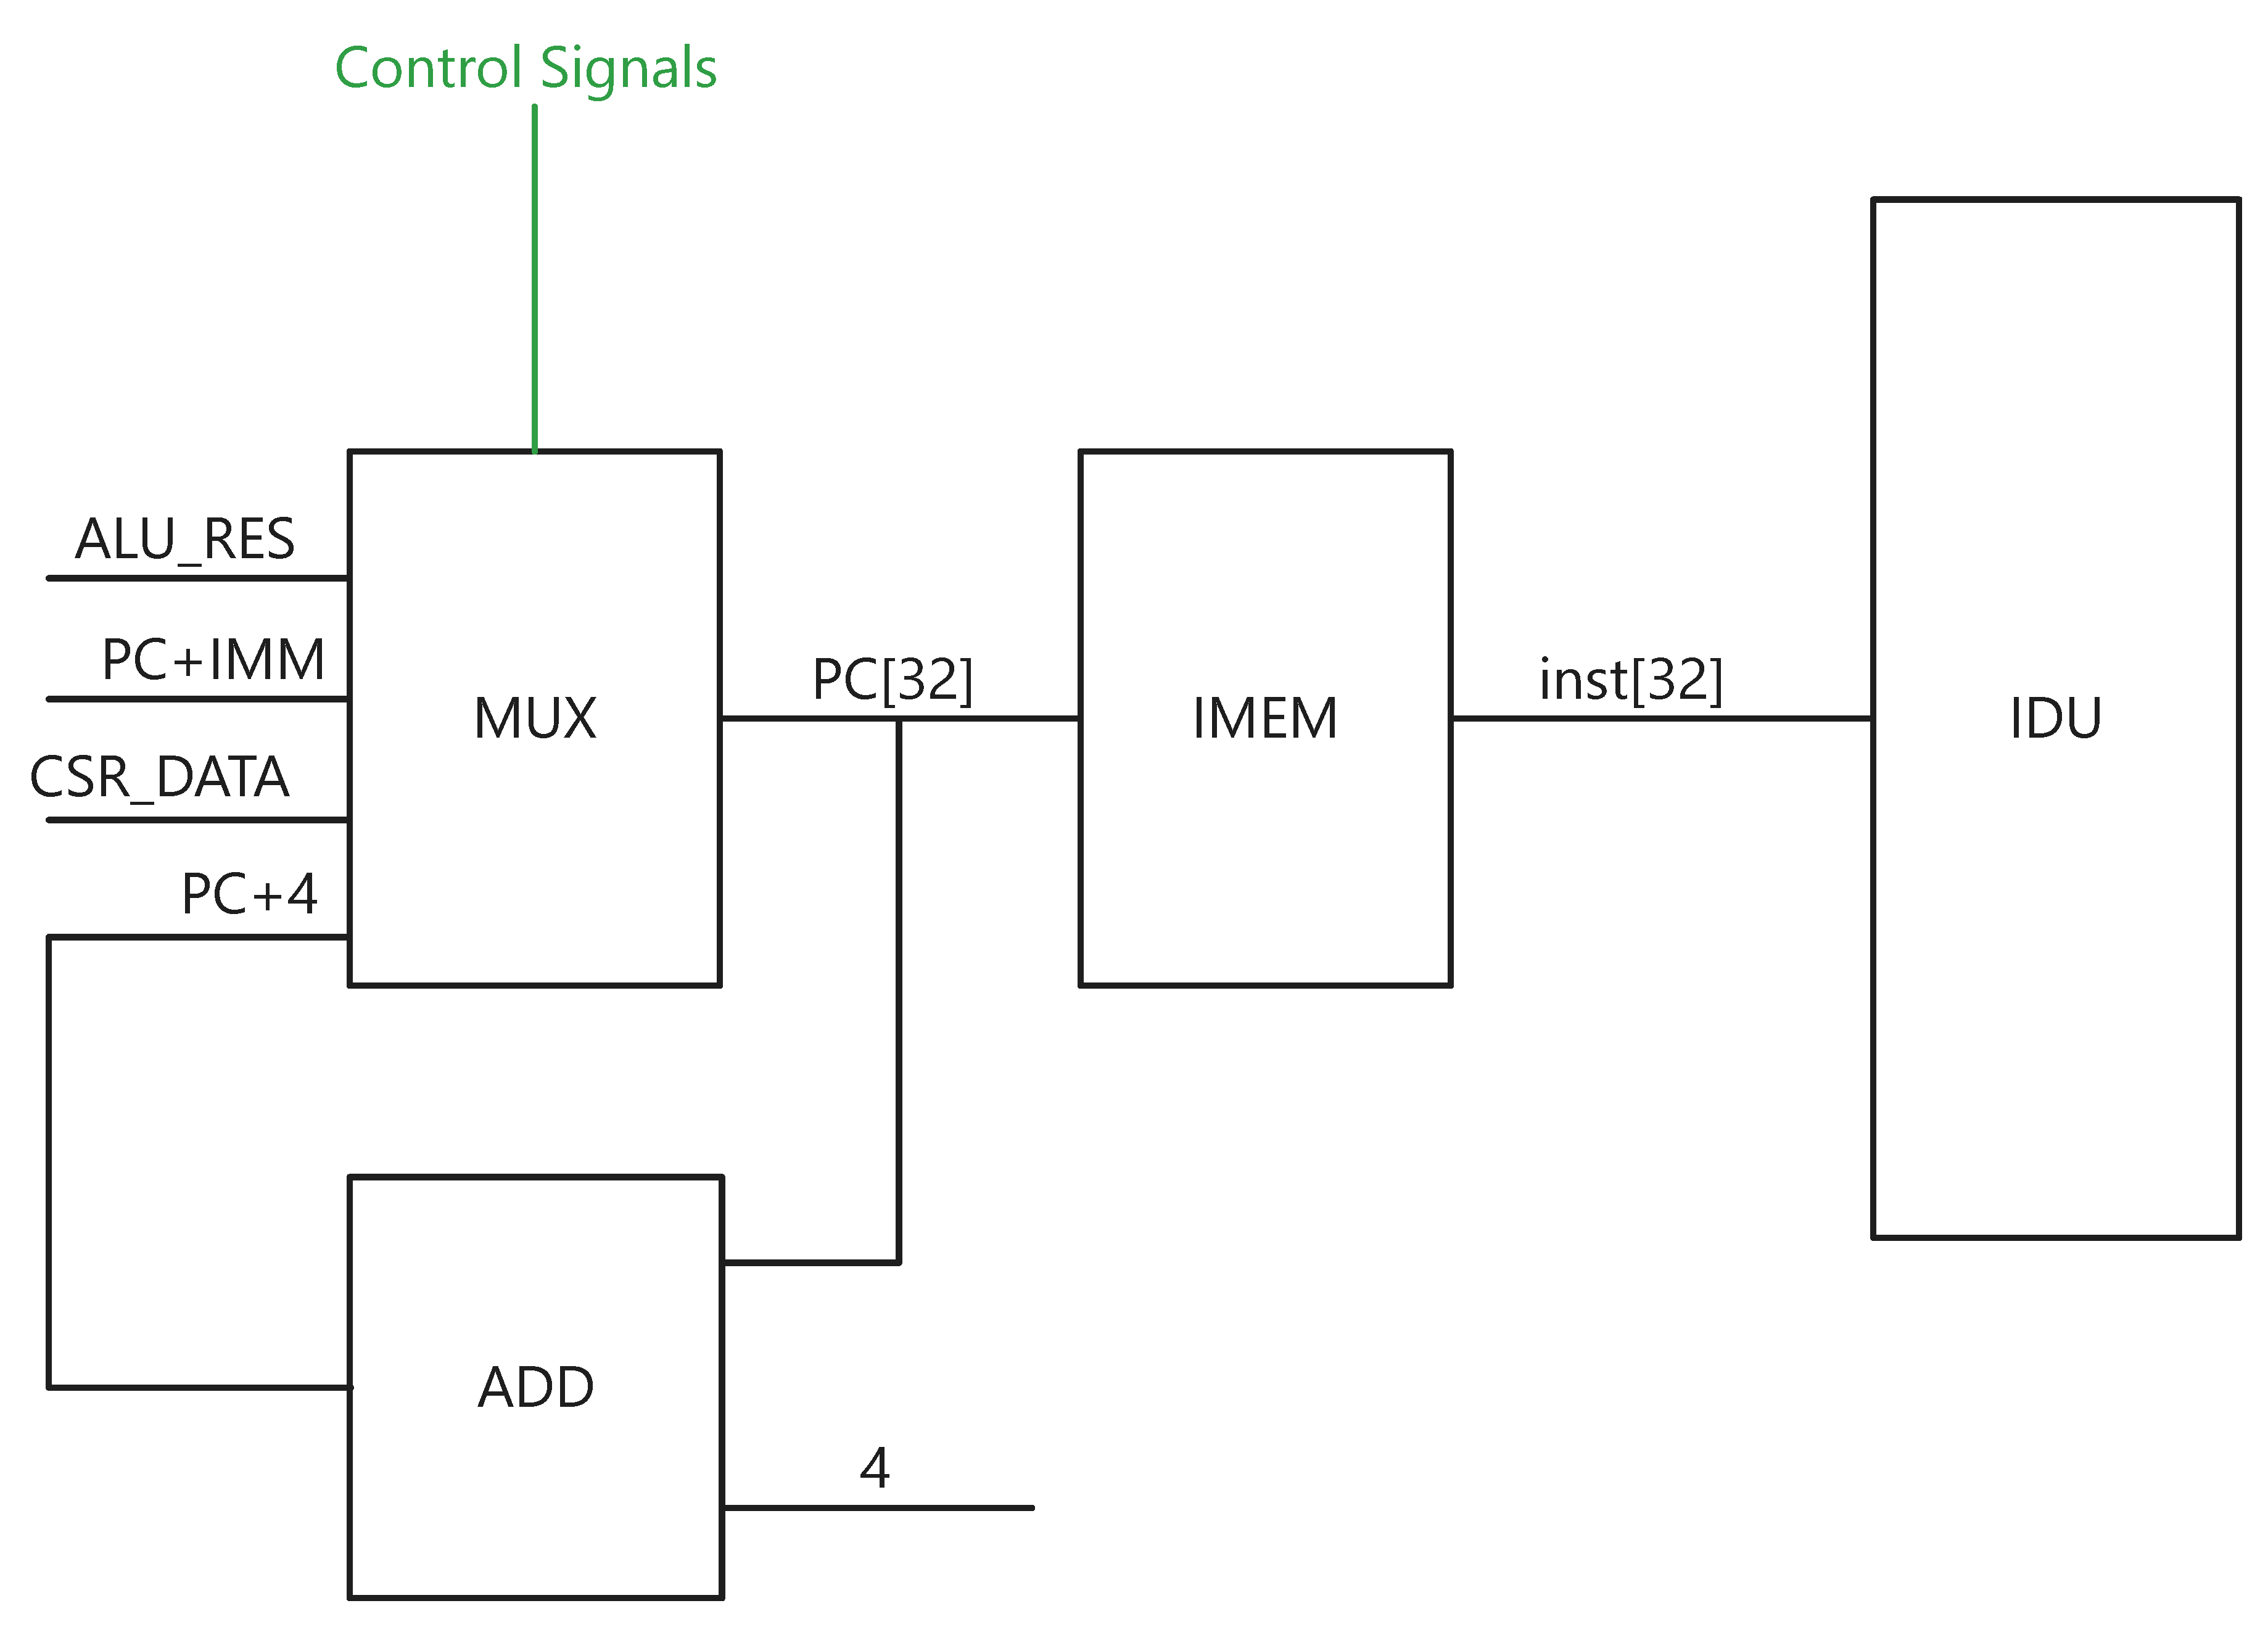
\includegraphics[width=0.6\textwidth]{image/ifu.pdf}
	\caption{取指单元设计图}
	\label{fig:ifu}
\end{figure}

如图\ref{fig:ifu}所示,程序计数器的选择有以下四种情况:

\begin{enumerate}[label={\arabic*)},itemsep=0pt, parsep=0pt]
	\item \textbf{ALU+RE}:这种选择用于实现寄存器跳转,将程序计数器设置为加法器运算结果所在的地址。这种机制允许程序根据寄存器中的值动态调整执行流程,从而实现复杂的控制结构;
	\item \textbf{PC+IMM}:这种选择用于实现PC相对跳转,将程序计数器设置为当前程序计数器与立即数的和所在的地址。这种机制允许程序在代码中进行相对位置的跳转,常用于条件分支和循环结构;
	\item \textbf{CSR\_DATA}:这种选择用于实现异常中断跳转,将程序计数器设置为控制状态寄存器值所在的地址。这种机制在处理异常和中断时非常关键,它允许程序发生异常和中断时跳转到预定义的处理程序,以及中断处理结束时返回程序;
	\item \textbf{PC+4}:这种选择用于实现静态跳转,将程序计数器设置为当前程序计数器与4的和所在的地址。这是程序正常执行时的默认行为,用于顺序执行下一条指令。
\end{enumerate}

这些PC选择机制共同确保了程序的灵活执行和高效控制流管理,为处理器在各种复杂场景下的稳定运行提供了基础。

\section{译码单元(IDU)}
译码单元(Instruction Decode Unit)负责将指令中携带的信息提取出来,这些信息被称为控制信号,后续将被传递给执行单元、访存单元和写回单元,用于进行结果选择。译码器的实现相对简单,如图\ref{fig:idu}所示,主要由译码器(Decoder)和控制信号单元(CSU)组成。

\begin{figure}[htbp]
	\centering
	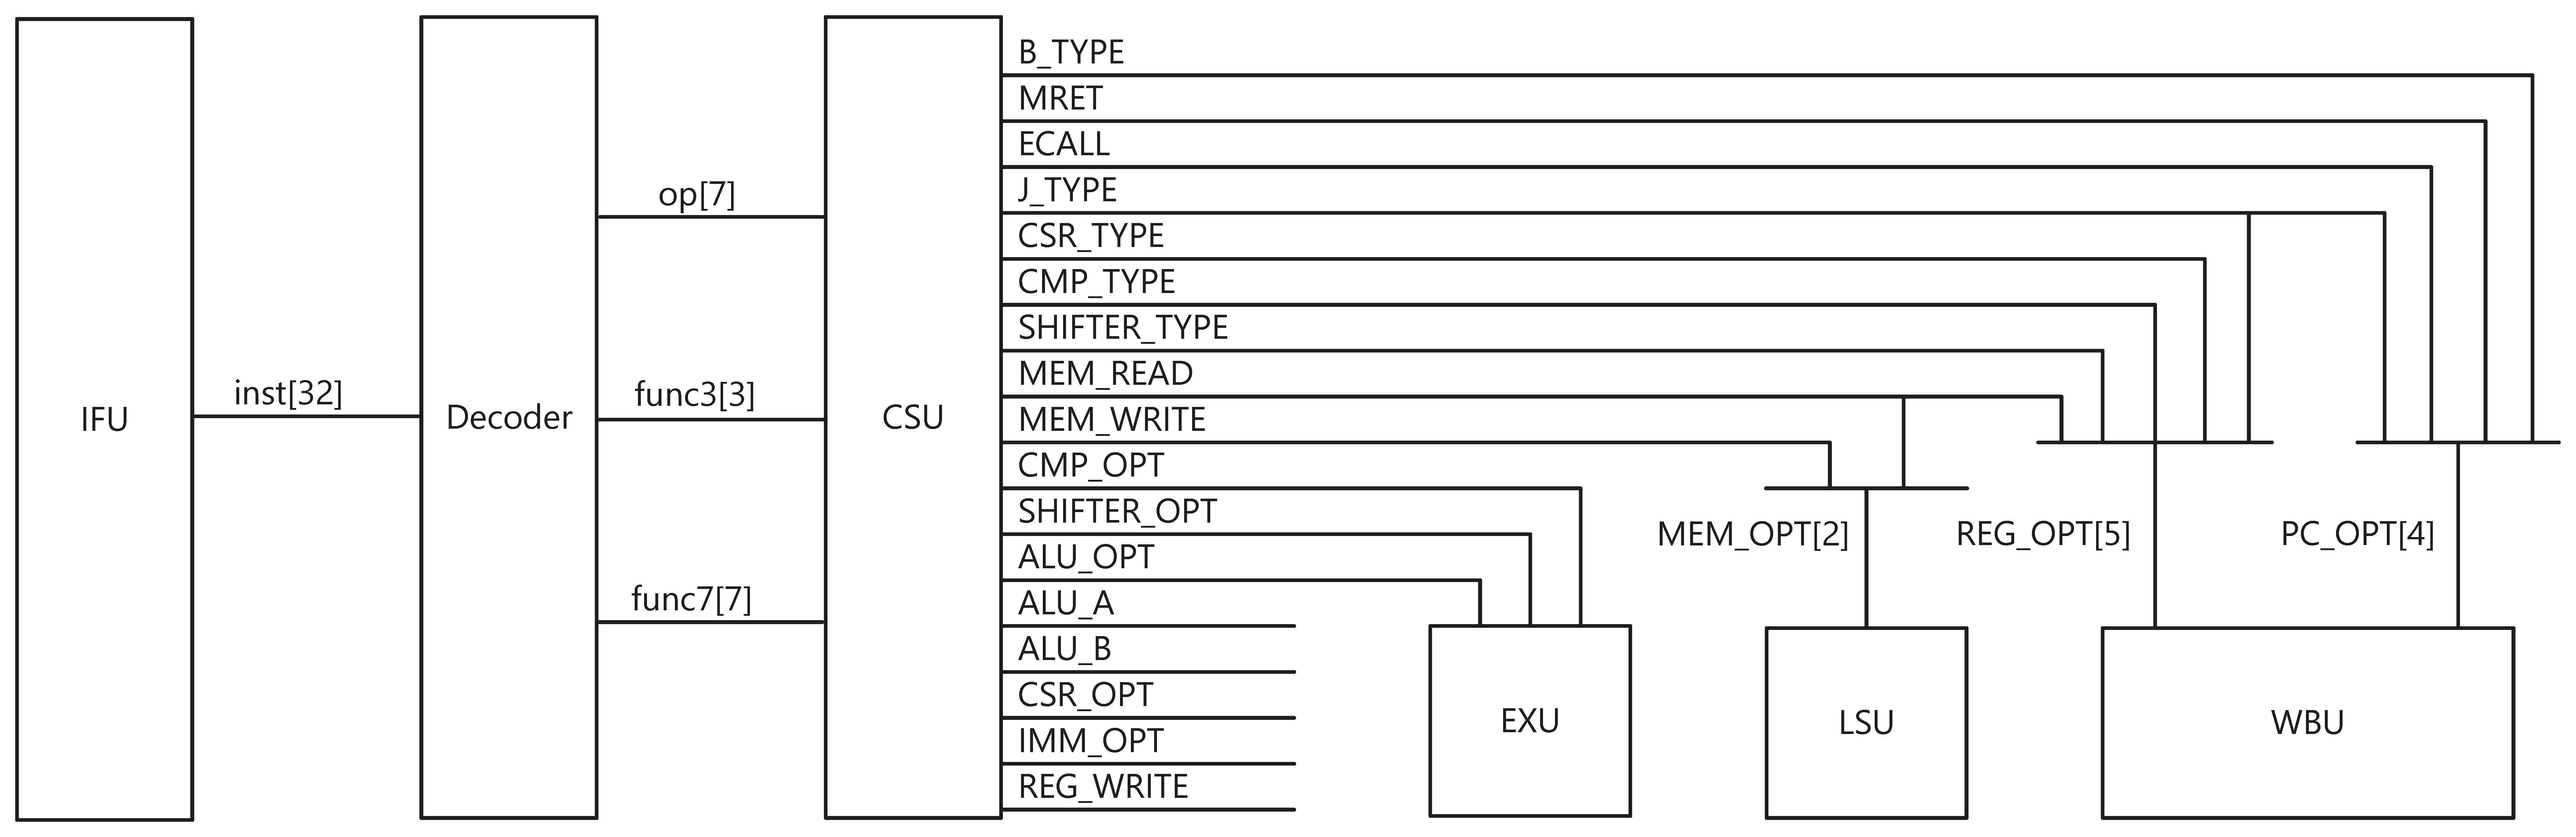
\includegraphics[width=0.9\textwidth]{image/idu.pdf}
	\caption{译码单元设计图}
	\label{fig:idu}
\end{figure}

\subsection{译码器}
译码器(Decoder)的任务是对接收到的指令进行初始译码,生成操作码(op)、功能码(func3和func7)、源寄存器(rs1和rs2)、目标寄存器(rd)以及立即数(imm)等关键信息。这些信息是后续处理的基础,其接口描述如表\ref{tab:decoder_interface}所示。

\begin{table}[htbp]
	\centering
	\caption{译码器接口描述表}
	\begin{tabularx}{\textwidth}{>{\centering\arraybackslash}X >{\centering\arraybackslash}X >{\centering\arraybackslash}X}
		\toprule
		\textbf{信号} & \textbf{位宽} & \textbf{描述} \\
		\midrule
		op          & 7           & 标识指令类型      \\
		func3       & 3           & 进一步细化指令具体操作 \\
		func7       & 7           & 扩展指令的功能     \\
		rs1         & 5           & 读寄存器1       \\
		rs2         & 5           & 读寄存器2       \\
		rd          & 5           & 写寄存器        \\
		\bottomrule
	\end{tabularx}
	\label{tab:decoder_interface}
\end{table}

\subsection{译码器}
控制信号单元(CSU)则负责将操作码(op)、功能码(func3和func7)转换为具体的控制信号。这些控制信号将指导处理器的各个模块如何协作以正确执行指令。CSU生成的控制信号包括ALU操作类型、数据通路选择信号等,其接口描述如表\ref{tab:csu_interface}所示。

\begin{table}[htbp]
	\centering
	\caption{控制信号单元接口描述表}
	\begin{tabularx}{\textwidth}{>{\centering\arraybackslash}X >{\centering\arraybackslash}X >{\centering\arraybackslash}X >{\centering\arraybackslash}X}
		\toprule
		\textbf{信号}  & \textbf{位宽} & \textbf{描述} & \textbf{下游} \\
		\midrule
		REG\_WRITE   & 1           & 是否将写入寄存器    & IDU         \\
		IMM\_OPT     & 6           & 立即数的扩展方式    & IDU         \\
		CSR\_OPT     & 2           & 选择CSR的值。    & IDU         \\
		ALU\_B       & 1           & 选择操作数B      & EXU         \\
		ALU\_A       & 1           & 选择操作数A      & EXU         \\
		ALU\_OPT     & 3           & 加法器的运算类型    & EXU         \\
		CMP\_OPT     & 4           & 比较器的运算类型    & EXU         \\
		SHIFTER\_OPT & 3           & 移位器的运算类型    & EXU         \\
		MEM\_OPT     & 2           & 存储器的读写类型    & LSU         \\
		REG\_OPT     & 5           & 写入寄存器堆的值    & WBU         \\
		PC\_OPT      & 4           & PC的更新方式     & WBU         \\
		\bottomrule
	\end{tabularx}
	\label{tab:csu_interface}
\end{table}

\section{执行单元(EXU)}
执行单元(Execution Unit)是处理器的核心组件之一,负责对操作数A和操作数B进行算术和逻辑运算,并将计算结果传递给访存单元和写回单元,以支持对存储器、寄存器和程序计数器的写操作。如图\ref{fig:exu}所示,执行单元主要由加法器(ALU)、比较器(CMP)和移位器(Shifter)组成。

\begin{figure}[htbp]
	\centering
	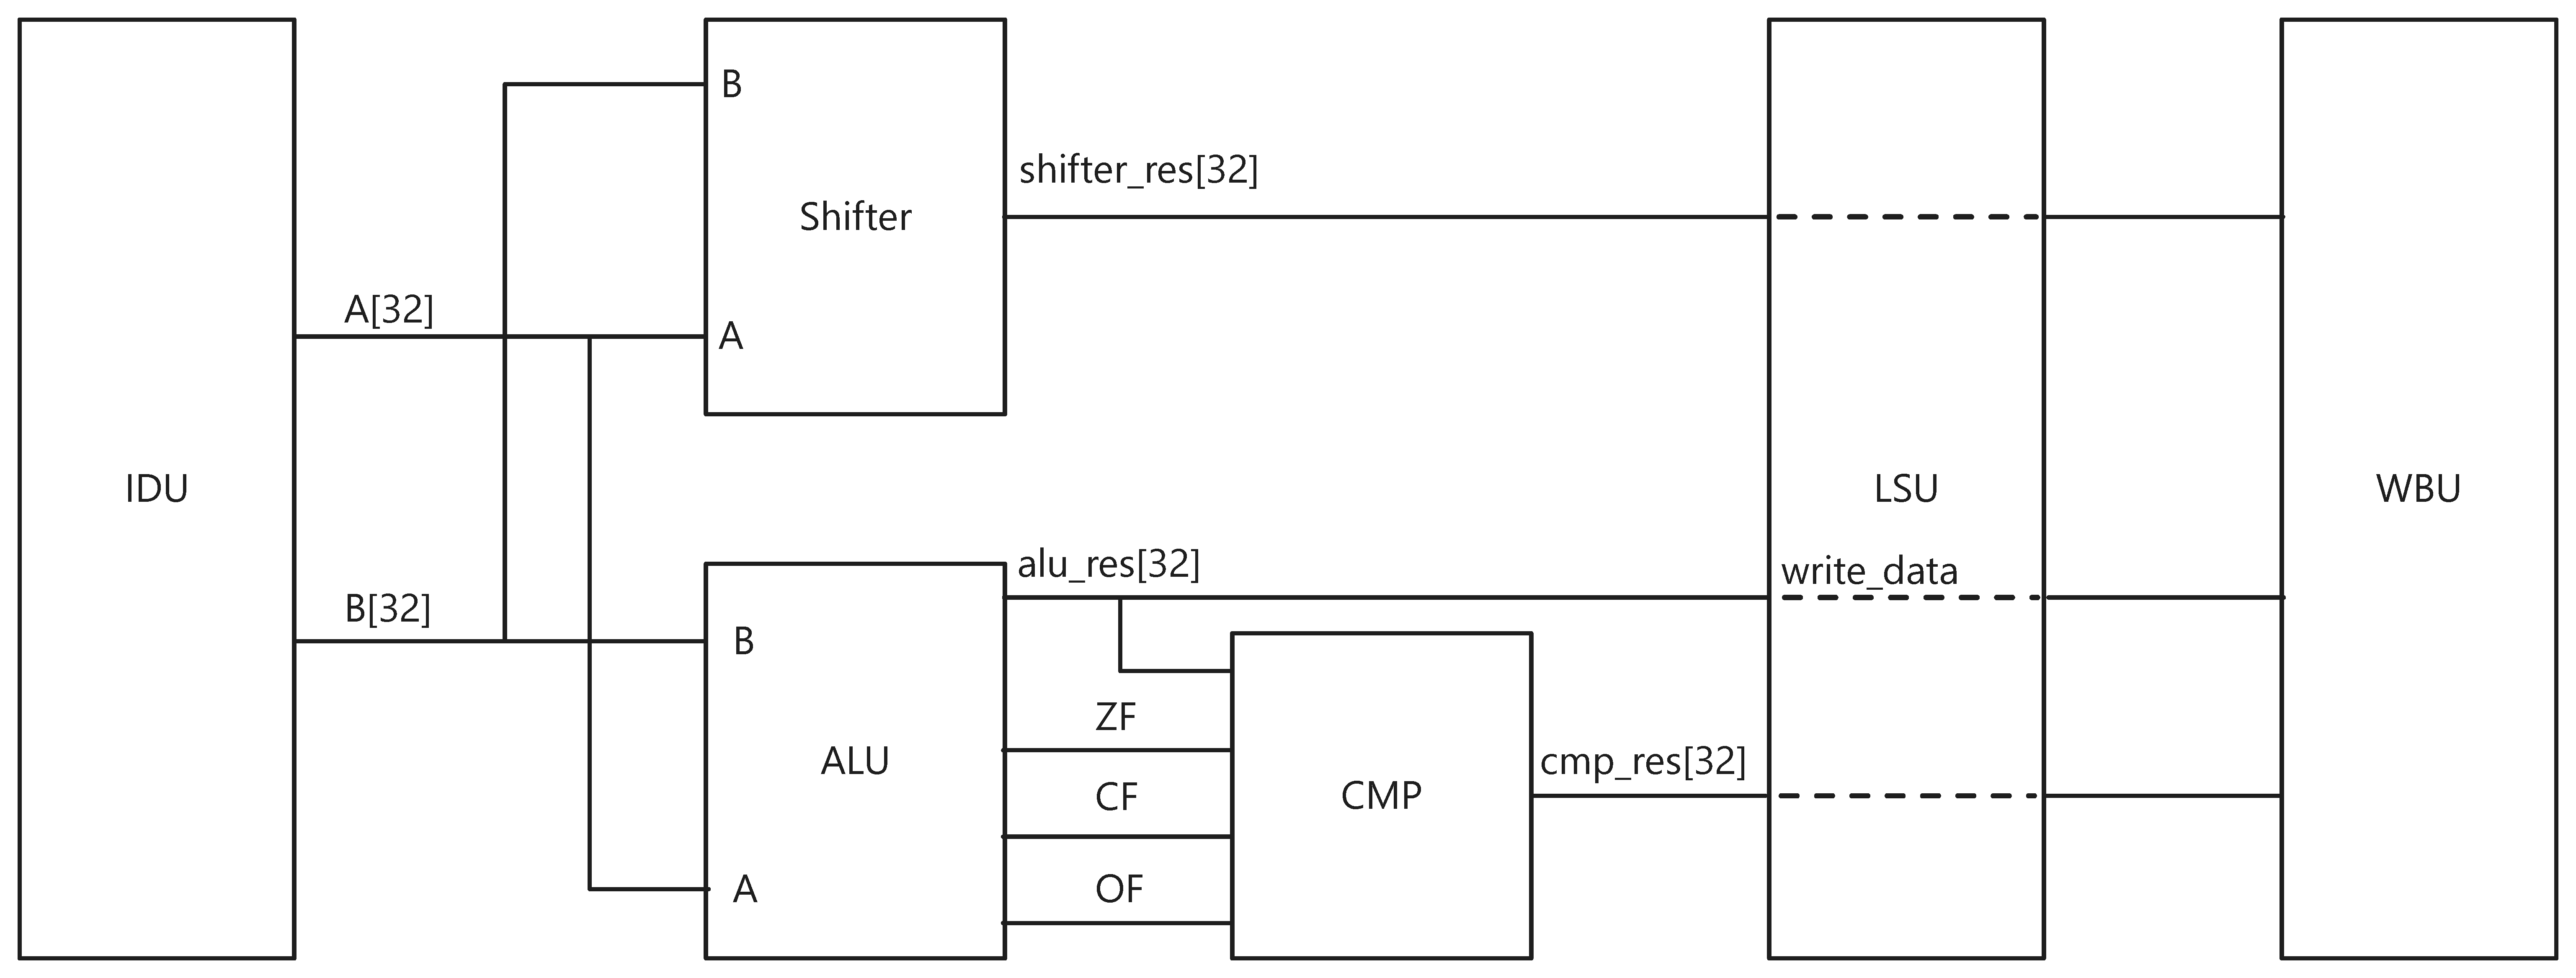
\includegraphics[width=0.9\textwidth]{image/exu.pdf}
	\caption{执行单元设计图}
	\label{fig:exu}
\end{figure}

\subsection{加法器}

加法器(ALU)是处理器执行单元的核心组件,用于执行基本的算术和逻辑运算。它能够高效地处理加法、减法,以及逻辑运算(如与、或、非等),确保数据的快速处理和准确计算。如图\ref{fig:alu}所示,该加法器设计采用经典的架构。输入信号有:两个32位的补码操作数,支持有符号数的运算;一个1位控制信号,用于决定执行加法或减法运算(控制信号为1,执行减法运算)。输出信号有:一个32位的运算结果,表示算术或逻辑运算的输出;一个1位的零标志符(ZF),用于指示运算结果是否为零;一个1位的进位标志符(CF),用于指示运算过程中是否发生进位;一个1位的溢出标志符(OF),用于检测有符号数运算中的溢出情况。

\begin{figure}[htbp]
	\centering
	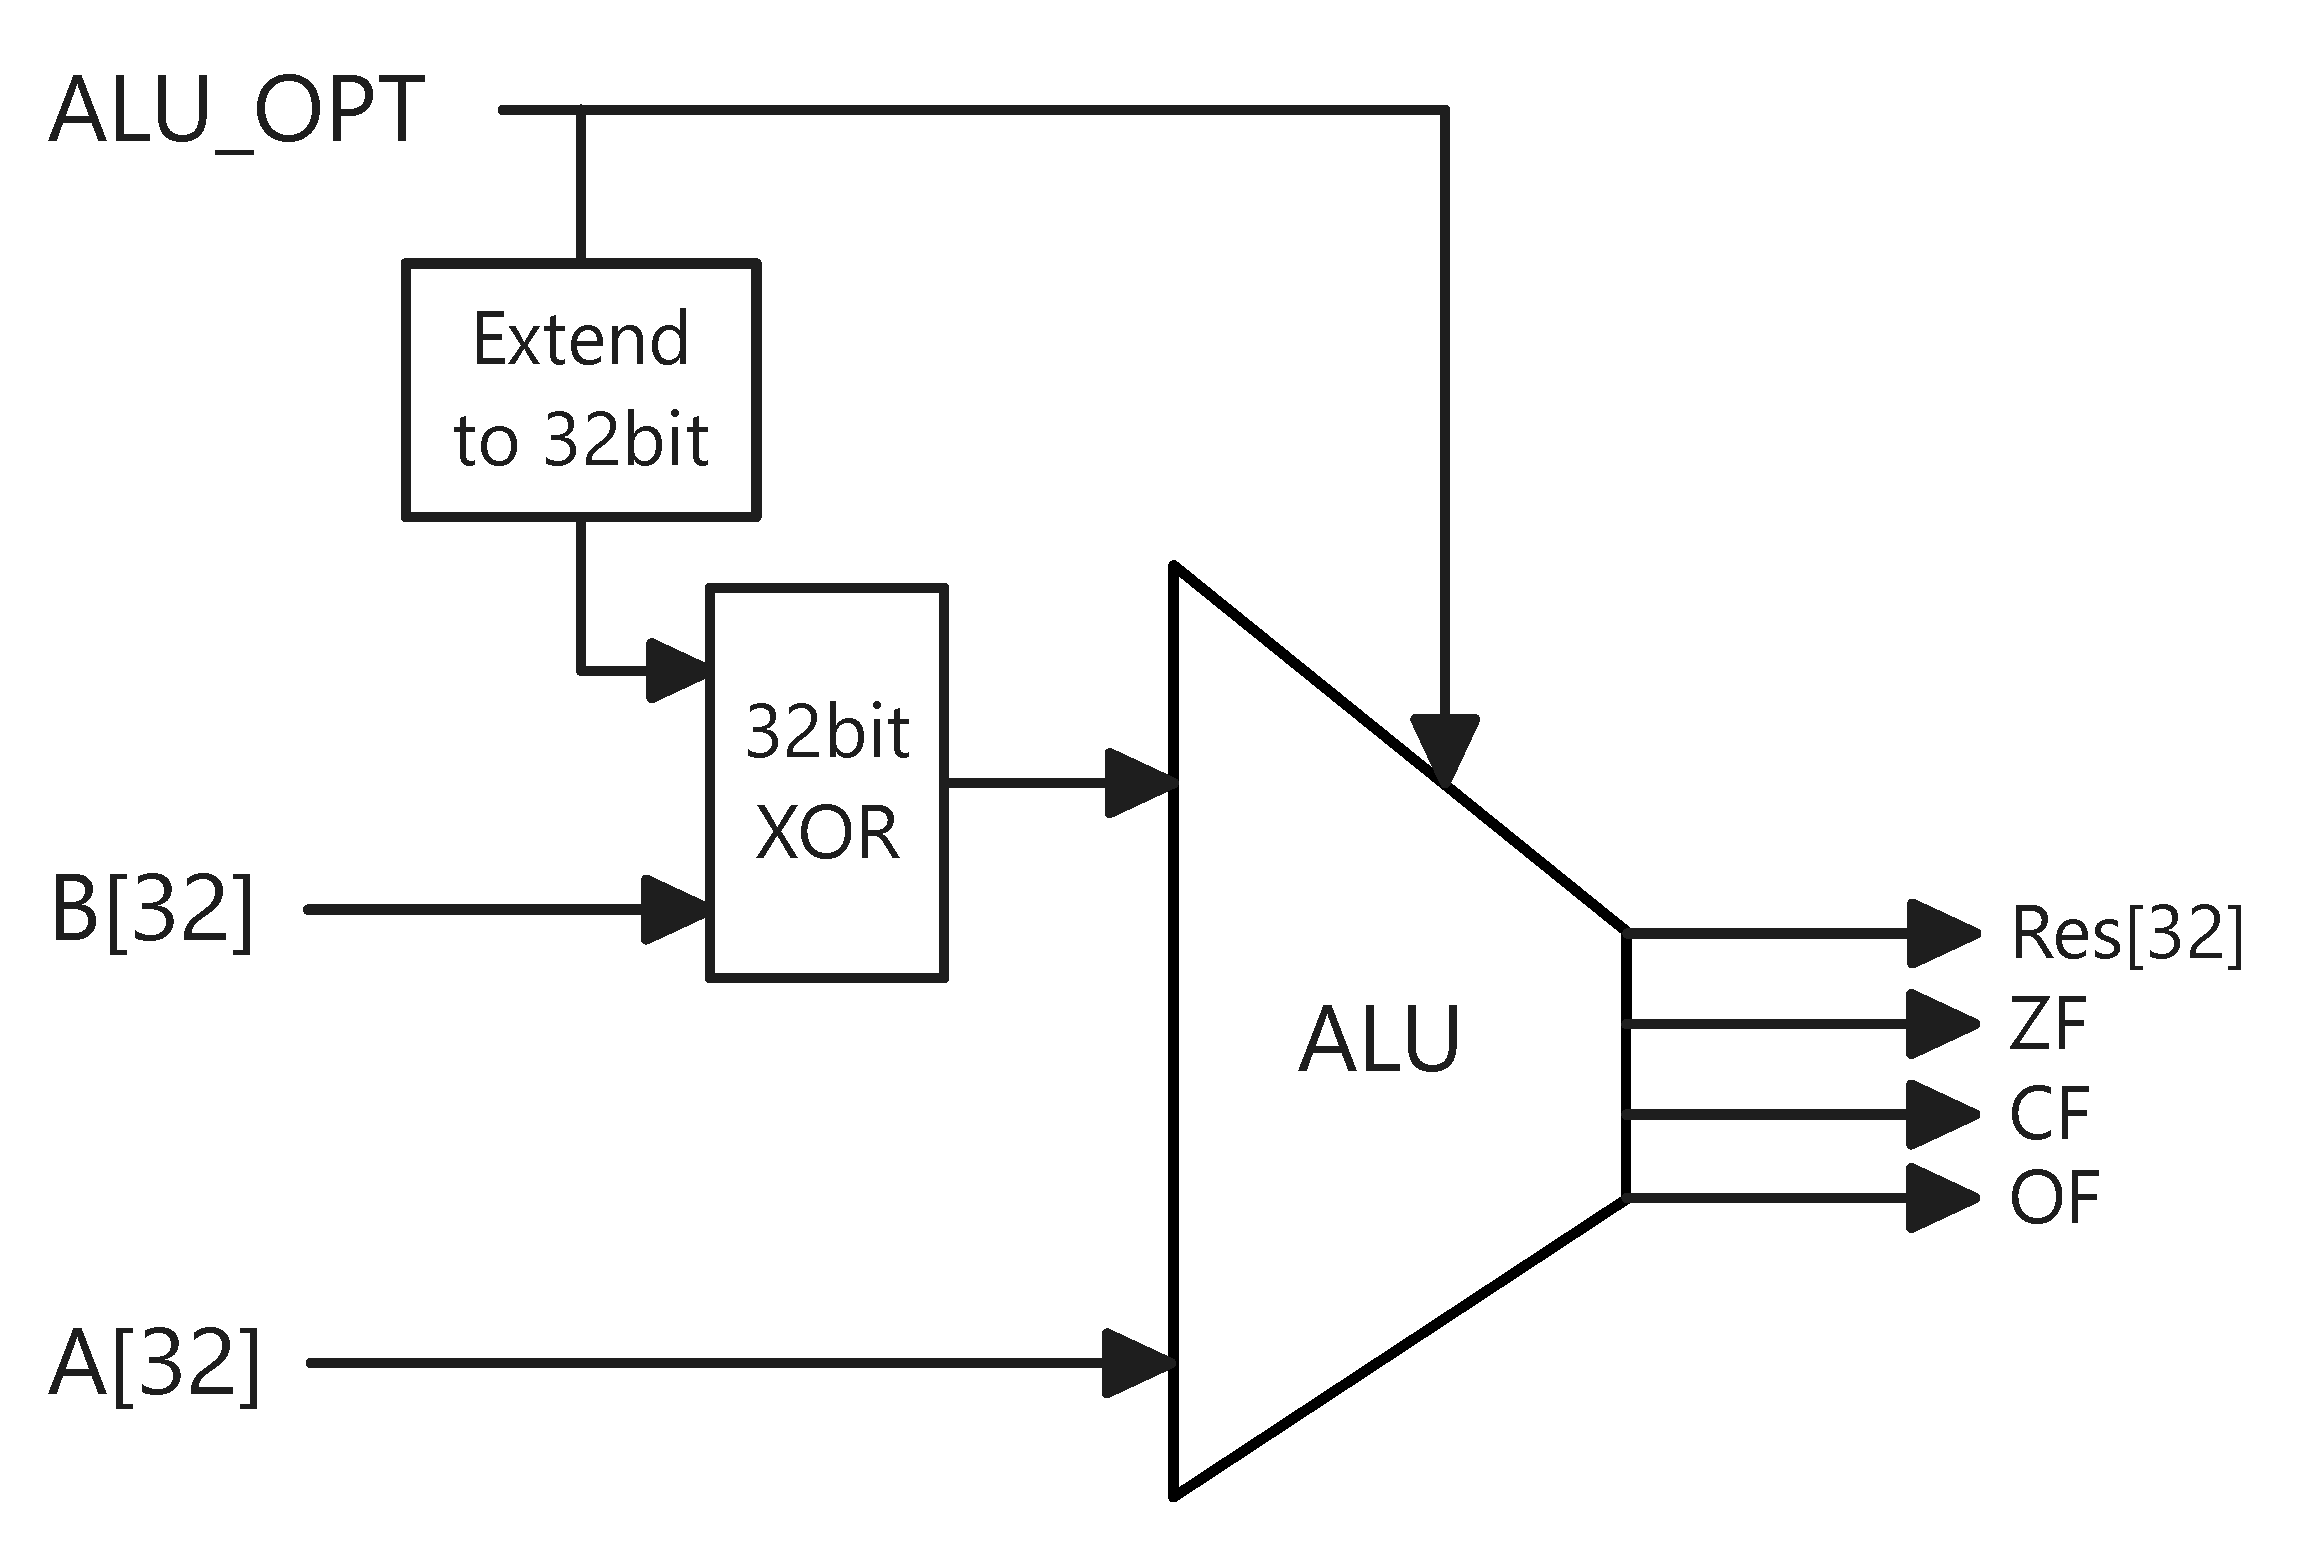
\includegraphics[width=0.5\textwidth]{image/alu.pdf}
	\caption{加法器设计图}
	\label{fig:alu}
\end{figure}

标志符在计算机系统中起着至关重要的作用,它们是处理器在执行指令后生成的信号,用于指示运算结果的特定状态。此外标志符还是比较器的输入,对于比较运算的判断十分重要。

\begin{enumerate}[label={\arabic*)},itemsep=0pt, parsep=0pt]
	\item \textbf{零标志符(ZF)}:指示运算结果是否为零。如果ZF为1,处理器可以判断某个操作的结果为零。ZF的运算参考公式\ref{eq:zf},其中$Res_i$表示运算结果的第$i$位。
	      \begin{equation}
		      ZF = \neg (Res_{31} \lor Res_{30} \lor \dots \lor Res_{0})
		      \label{eq:zf}
	      \end{equation}
	\item \textbf{进位标志符(CF)}:指示无符号数加法中的溢出或减法中的借位。如果CF为1,说明无符号运算发生溢出。CF的运算参考公式\ref{eq:cf},其中$C_i$表示第$i$位的进位信息。
	      \begin{equation}
		      CF = C_{32} \oplus C_{0}
		      \label{eq:cf}
	      \end{equation}
	\item \textbf{溢出标志符(OF)}:指示有符号数运算中的溢出。如果OF为1,说明有符号运算发生溢出。OF的运算参考公式\ref{eq:of}。
	      \begin{equation}
		      OF = C_{32} \oplus C_{31}
		      \label{eq:of}
	      \end{equation}
\end{enumerate}

除了最基本的加减法运算之外,加法器还应该支持逻辑运算和移位。将ALU\_OPT扩充至3位,从而能够支持更多的运算类型,扩充后的接口描述如表\ref{tab:alu_option}所示。

\begin{table}[htbp]
	\centering
	\caption{ALU\_OPT接口描述表}
	\begin{tabularx}{\textwidth}{>{\centering\arraybackslash}X >{\centering\arraybackslash}X >{\centering\arraybackslash}X}
		\toprule
		\textbf{ALU\_OPT} & \textbf{功能} & \textbf{操作}  \\
		\midrule
		000               & 加法          & $A+B$        \\
		001               & 减法          & $A-B$        \\
		010               & 取反          & $\neg A$     \\
		011               & 与           & $A \land B$  \\
		100               & 或           & $A \lor B$   \\
		101               & 异或          & $A \oplus B$ \\
		\bottomrule
	\end{tabularx}
	\label{tab:alu_option}
\end{table}

\subsection{比较器}
比较器(CMP)是处理器执行单元中的关键器件,用于执行条件比较操作。它能够高效地判断两个操作数之间的关系,为条件分支指令提供依据。输入信号包括来自加法器的四个标志位(SF、ZF、CF和OF),这些标志位用于计算比较结果。此外,比较器还接收一个4位的控制信号(CMP\_OPT),用于决定执行何种比较运算。CMP\_OPT的接口描述如表\ref{tab:cmp_option}所示。

\begin{table}[htbp]
	\centering
	\caption{CMP\_OPT接口描述表}
	\begin{tabularx}{\textwidth}{>{\centering\arraybackslash}X >{\centering\arraybackslash}X >{\centering\arraybackslash}X}
		\toprule
		\textbf{CMP\_OPT} & \textbf{功能} & \textbf{逻辑}                         \\
		\midrule
		0001或1001         & ==          & $ZF = 1$                            \\
		0010或1010         & !=          & $ZF = 0$                            \\
		0011              & <(有符号)      & $SF \oplus OF$                      \\
		0100              & <=(有符号)     & $(SF \oplus OF) \lor (ZF = 1)$      \\
		0101              & >(有符号)      & $\neg (SF \oplus OF)$               \\
		0110              & >=(有符号)     & $\neg (SF \oplus OF) \lor (ZF = 1)$ \\
		1011              & <(无符号)      & $\neg CF$                           \\
		1100              & <=(无符号)     & $\neg CF \lor (ZF = 1)$             \\
		1101              & >(无符号)      & $CF \land (ZF = 0)$                 \\
		1110              & >=(无符号)     & $CF$                                \\
		\bottomrule
	\end{tabularx}
	\label{tab:cmp_option}
\end{table}

\subsection{移位器}
移位器(Shifter)是处理器执行单元中的重要模块,用于执行数据的移位操作。它能够高效地处理多种类型的移位运算,包括逻辑左移、逻辑右移和算术右移,这些操作在数据处理和数值计算中非常常见。输入信号包括一个32位的被移数与32位的移数,这两个操作数用于计算移位结果。此外,移位器还会接收一个2位的控制信号(SHIFTER\_OPT),用于决定执行何种移位运算。SHIFTER\_OPT的接口描述表如\ref{tab:shifter_option}所示。

\begin{enumerate}[label={\arabic*)},itemsep=0pt, parsep=0pt]
	\item \textbf{逻辑左移(ZF)}:将操作数的各位向左移动指定的位数,空出的低位填充零。
	\item \textbf{进位标志符(CF)}:将操作数的各位向右移动指定的位数,空出的高位填充零。
	\item \textbf{溢出标志符(OF)}:将操作数的各位向右移动指定的位数,空出的高位填充操作数的符号位(最高位),以保持有符号数的符号不变。
\end{enumerate}

\begin{table}[htbp]
	\centering
	\caption{SHIFTER\_OPT接口描述表}
	\begin{tabularx}{\textwidth}{>{\centering\arraybackslash}X >{\centering\arraybackslash}X}
		\toprule
		\textbf{SHIFTER\_OPT} & \textbf{功能} \\
		\midrule
		00或01                 & 逻辑左移        \\
		10                    & 逻辑右移        \\
		11                    & 算术右移        \\
		\bottomrule
	\end{tabularx}
	\label{tab:shifter_option}
\end{table}

\section{访存单元(LSU)}
访存单元(Load Store Unit)是处理器与存储器交互的关键模块,其设计严格遵循加载-存储(Load-Store)架构原则,负责对存储器进行读写操作。如图\ref{fig:lsu}所示,写操作的数据来源于寄存器,写地址来源于执行单元,而读取的数据则被发送到写回单元。

为了降低访问延迟并提高性能,现代处理器中的LSU通常采用多种优化技术,如高速缓存(Cache)、预取(Prefetching)和多端口存储器。这些技术能够显著减少存储器访问延迟,提高数据传输效率,从而提升处理器的主频和IPC(每周期指令数)。然而,在本章中,仅探讨单周期处理器的设计,因此访存单元采用最简单的存取方案。关于高速缓存优化的详细讨论将在第4章中进行,届时将介绍如何通过缓存技术进一步提升访存单元的性能。

\begin{figure}[htbp]
	\centering
	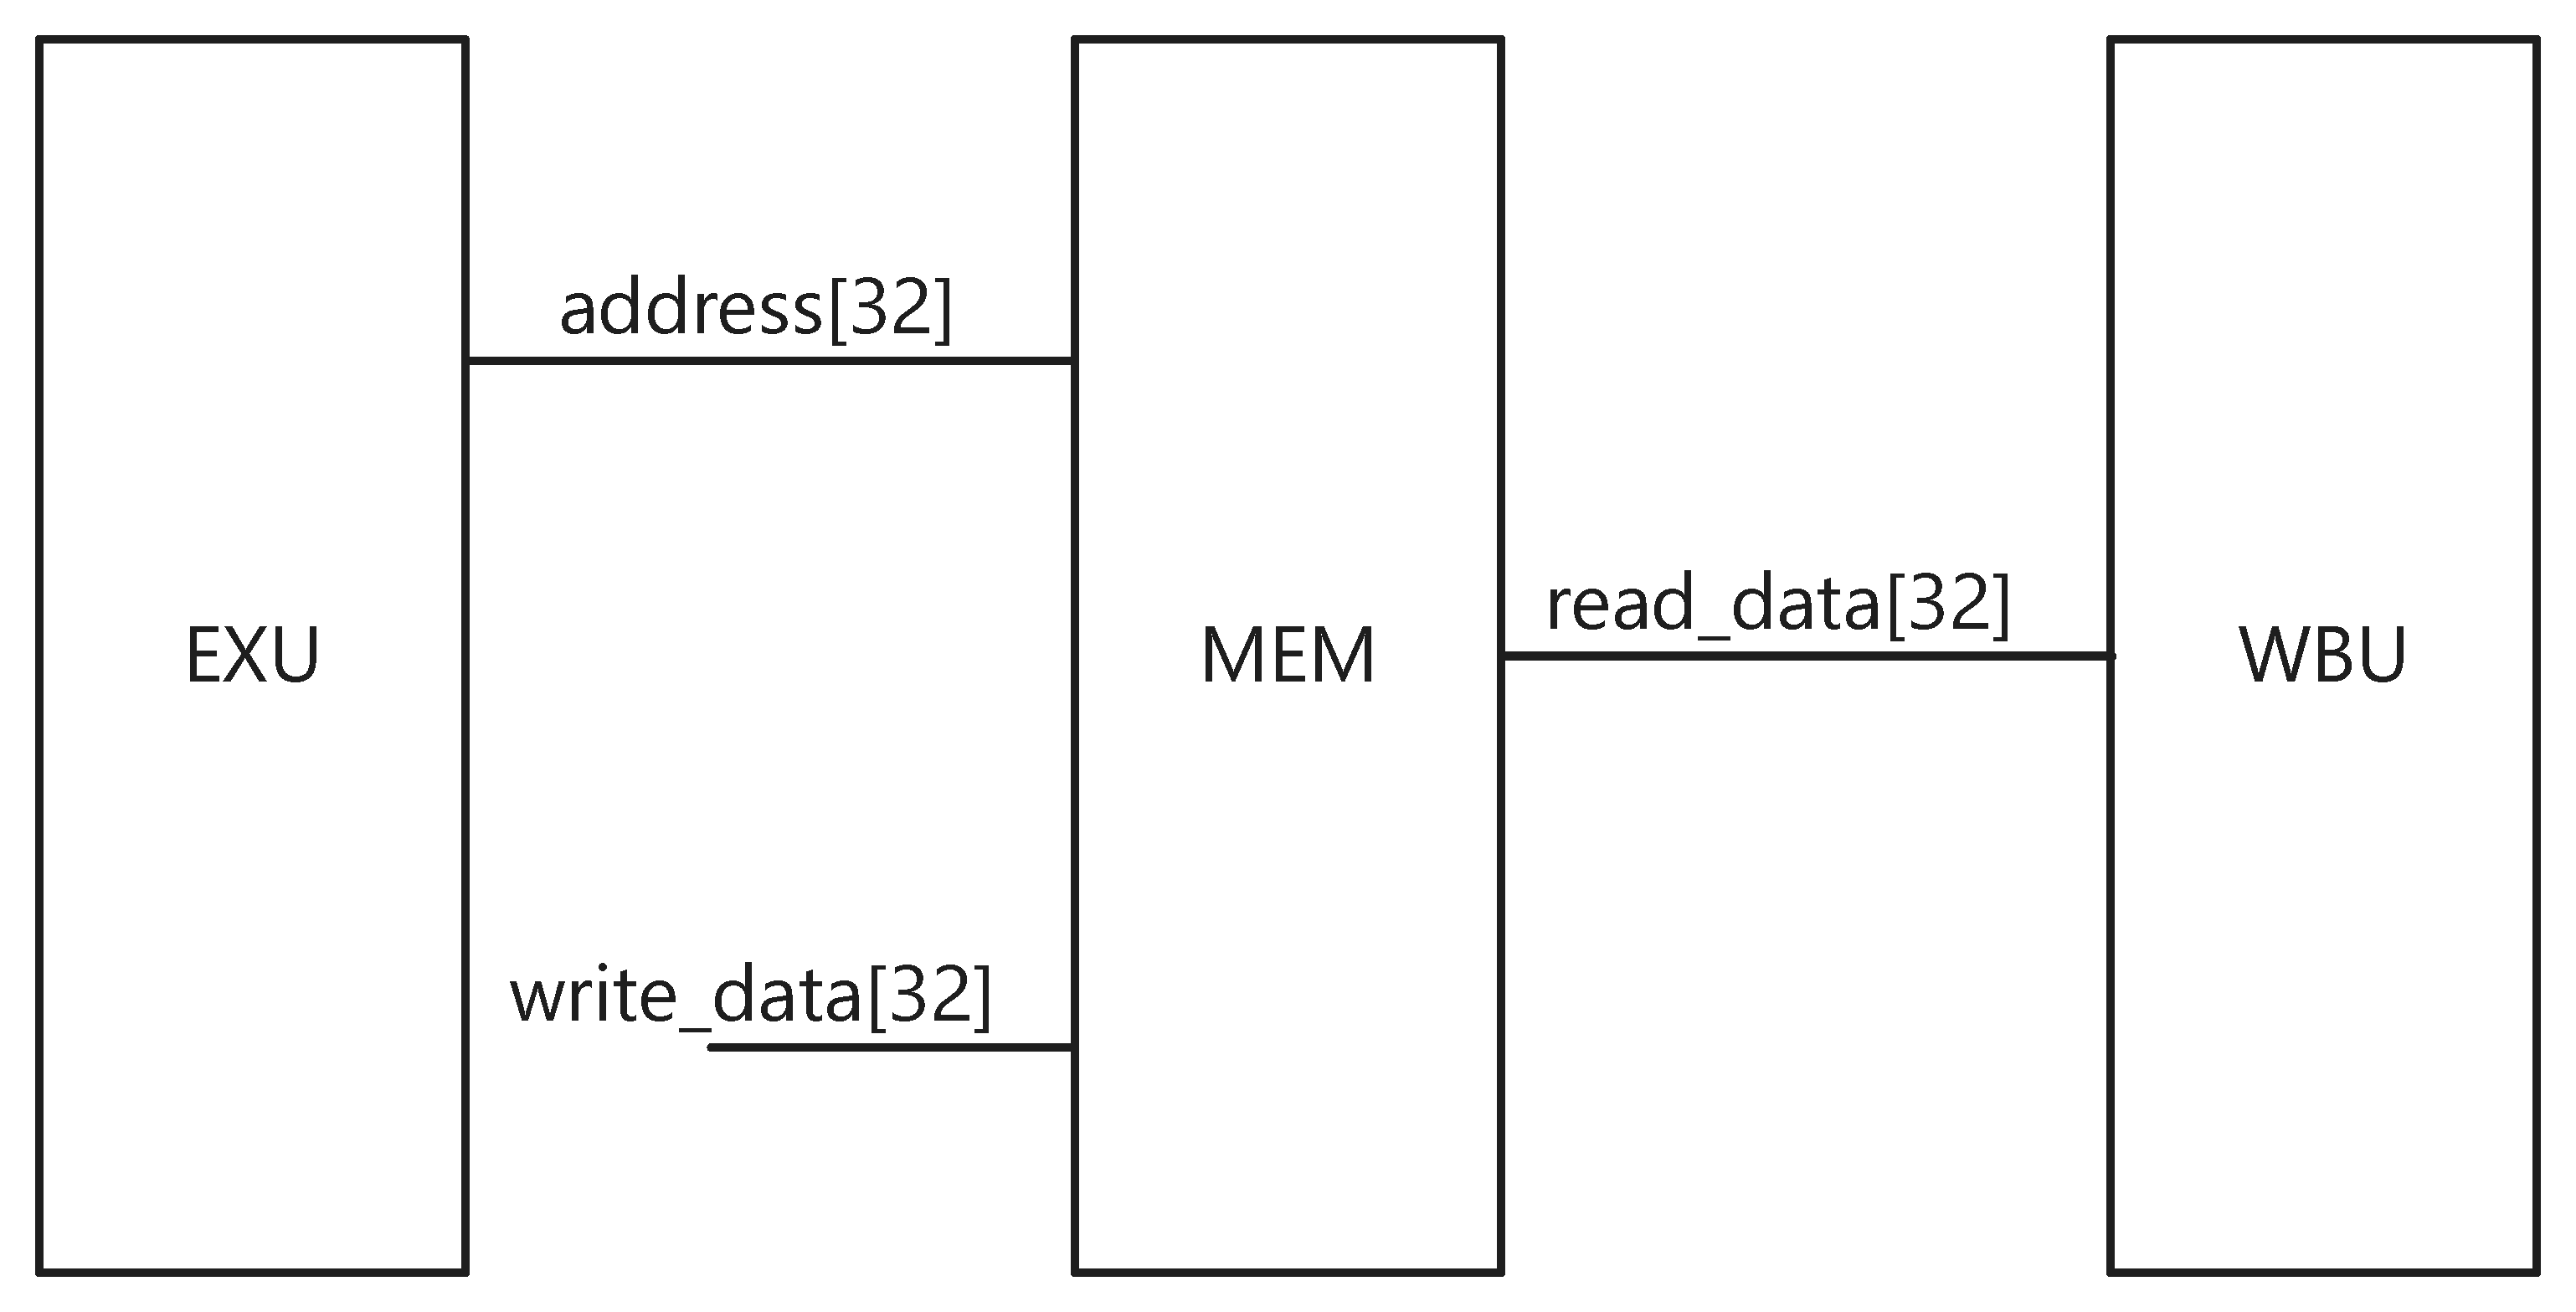
\includegraphics[width=0.6\textwidth]{image/lsu.pdf}
	\caption{访存单元设计图}
	\label{fig:lsu}
\end{figure}

\section{写回单元(WBU)}
写回单元(Write Back Unit,WBU)是微处理器五个核心单元中的最后一个单元,其主要职责是将处理结果写入寄存器堆,并更新程序计数器。WBU确保了运算结果的最终存储和程序流程的正确推进,其设计的高效性和可靠性直接影响处理器的整体性能和稳定性。

写回寄存器的值由控制信号REG\_OPT确定,该控制信号的位宽为5位,由译码单元输出。更新程序计数器的值由控制信号PC\_OPT确定,该控制信号的位宽为4位,由译码单元和执行单元共同输出。表\ref{tab:reg_option}和表\ref{tab:pc_option}是控制信号REG\_OPT和PC\_OPT的详细描述。

\begin{table}[htbp]
	\centering
	\caption{REG\_OPT接口描述表}
	\begin{tabularx}{\textwidth}{>{\centering\arraybackslash}X >{\centering\arraybackslash}X}
		\toprule
		\textbf{REG\_OPT} & \textbf{写入寄存器堆的值} \\
		\midrule
		00000             & 加法器结果             \\
		00001             & PC+4              \\
		00010             & CSR的值             \\
		00100             & 比较器结果             \\
		01000             & 访存数据              \\
		10000             & 移位器结果             \\
		\bottomrule
	\end{tabularx}
	\label{tab:reg_option}
\end{table}

\begin{table}[htbp]
	\centering
	\caption{PC\_OPT接口描述表}
	\begin{tabularx}{\textwidth}{>{\centering\arraybackslash}X >{\centering\arraybackslash}X}
		\toprule
		\textbf{PC\_OPT} & \textbf{更新PC的值} \\
		\midrule
		0000             & PC+4            \\
		0001             & PC+IMM          \\
		0010             & CSR的值(MRET)     \\
		0100             & CSR的值(ECALL)    \\
		1000             & 加法器结果           \\
		\bottomrule
	\end{tabularx}
	\label{tab:pc_option}
\end{table}

\section{本章小结}
本章着重阐述了RISC-V单周期处理器的设计方法,采用RV32I指令集,该指令集支持RISC-V架构的基本功能。文中依次详细介绍了处理器五个核心单元的设计,分别为指令取指单元(IFU)、指令译码单元(IDU)、执行单元(EXU)、访存单元(LSU)和写回单元(WBU)。IFU负责依据程序计数器(PC)从存储器中读取指令,并将其传递至IDU;IDU承担将指令译码为多种控制信号的任务,为后续处理单元提供必要的支持;EXU包含加法器、比较器和移位器,用于执行算术和逻辑运算,并将结果传递给后续单元;LSU实现存储器的读写操作;WBU则负责更新寄存器堆和程序计数器(PC)。这种模块化设计明确划分了各单元的职责,不仅降低了设计的复杂度,还便于后续的技术优化,例如总线架构、高速缓存策略和片上系统集成等。
